% Adaptive Arbitration in Command Space for Target Following under Passability Mismatch
% Revised manuscript with substantive changes highlighted.
\documentclass[letterpaper, 10 pt, conference]{ieeeconf}
\IEEEoverridecommandlockouts
\overrideIEEEmargins
\setlength{\topmargin}{-14pt}
\usepackage{amsmath,amssymb,amsfonts}
\usepackage{graphicx}
\usepackage{stfloats}
\usepackage{booktabs}
\usepackage{multirow}
\usepackage{array}
\usepackage[table]{xcolor}
\usepackage{url}
\usepackage{pifont}
\usepackage[hidelinks]{hyperref}
\usepackage{placeins}
\newcommand{\uF}{u_{F}}
\newcommand{\uA}{u_{A}}
\newcommand{\alphaeff}{\alpha_{\mathrm{eff}}}
\newcommand{\rFdir}{\rho_F}
\newcommand{\rAdir}{\rho_A}
\newcommand{\darisk}{\Delta \alpha_r}
\newcommand{\msec}{\,\mathrm{m/s}}
\newcommand{\ms}[2]{\ensuremath{#1{\pm}#2}}
\newcommand{\bms}[2]{\ensuremath{\mathbf{#1{\pm}#2}}}

\newcommand{\rev}[1]{\textcolor{blue}{#1}}
\begin{document}
\title{\LARGE \bf
\rev{Adaptive Arbitration in Command Space for Target Following under Passability Mismatch}}
\author{
\thanks{}%
\thanks{}}
\maketitle
\thispagestyle{empty}
\pagestyle{empty}

\begin{abstract}
A legged robot following a person through clutter may encounter passages that the person can traverse but the robot cannot safely negotiate. This passability mismatch creates conflicts between target recovery and obstacle clearance. \rev{We propose an adaptive arbitration framework in command space that coordinates analytic forward--yaw following and pretrained lateral avoidance proposals.} A learned arbitration gate adjusts their relative authority based on risk while keeping both experts and the locomotion policy fixed, \rev{concentrating learning on behavioral coordination}. \rev{On the held-out evaluation, the method achieves 95.3\% task success at 0.60 m/s, 20\% above the maximum training speed.} With onboard target detection and stereo depth, it succeeds in 37 of 40 hardware trials across staggered-row and sharp-turn corridors. \rev{Comparisons with additive fusion, fixed authority, and monolithic PPO support the value of context-dependent authority allocation in the tested conditions.}
\end{abstract}

\section{Introduction}
A moving person can pass through gaps that a legged robot's gait envelope cannot safely traverse (Fig.~\ref{fig:teaser}). This \emph{passability mismatch} couples collision avoidance with target retention: tracking the person can reduce clearance, whereas avoidance can cause target loss. We study how to allocate authority between Follow and Avoid proposals as this conflict changes.

\rev{The proposed arbitration framework combines analytic Follow and learned Avoid proposals in orthogonal command subspaces (Fig.~\ref{fig:system}).} The gate uses obstacle risk along each proposal's direction to allocate authority between them. The experts and the pretrained locomotion policy remain fixed, \rev{concentrating learning on their coordination}.

\begin{figure}[t]
\centering
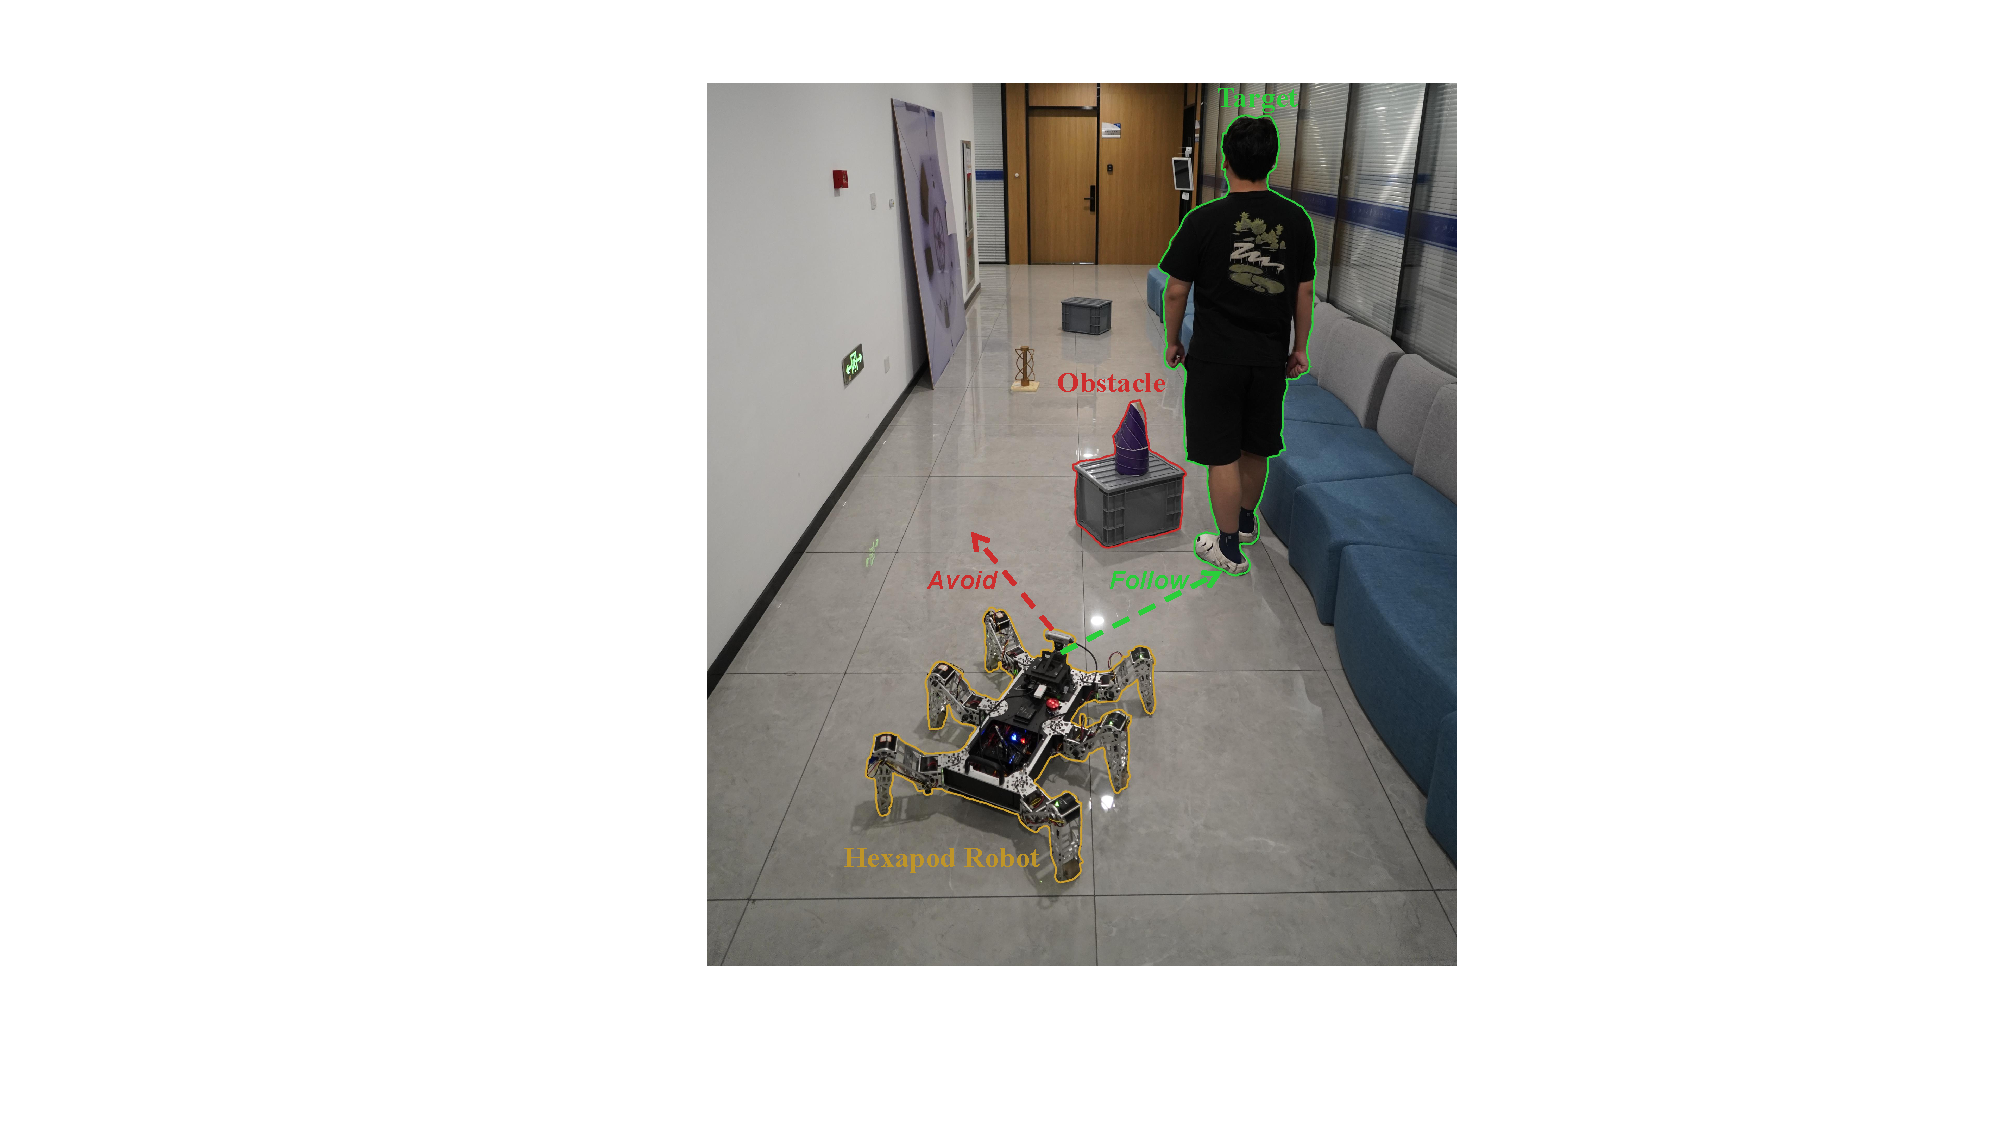
\includegraphics[width=0.80\columnwidth]{figs/fig1_real_scene.pdf}
\caption{Real corridor setting for hexapod target following in clutter. Gaps passable by the target may be too narrow for the robot's leg-inclusive envelope, creating a conflict between target recovery and collision avoidance.}
\label{fig:teaser}
\end{figure}
The hexapod supports the lateral motion required by this decomposition, while its fixed 18-joint locomotion policy realizes the commands. \rev{Arbitration uses high-level velocities without hexapod-specific joint observations.} Staggered rows provide a controlled stress test: successive obstacle rows require sidestepping while the target advances.

\noindent\textbf{Contributions.}
\begin{itemize}
\item \rev{\textbf{Command-space formulation of passability mismatch.} We formulate the conflict between moving-target retention and local collision avoidance as continuous authority allocation in command space.}
\item \rev{\textbf{Risk-conditioned adaptive arbitration.} A risk-conditioned gate blends fixed Follow and Avoid proposals in orthogonal command subspaces. The bounded raw convex blend passes through shared post-processing and fixed locomotion.}
\item \rev{\textbf{Controlled validation of arbitration.} Comparisons among arbitration variants reuse the same experts, and the inference ablation reuses the same checkpoint, keeping expert and locomotion capability fixed. Held-out simulation and hardware trials quantify the safety--following trade-off.}
\end{itemize}

\section{Related Work}
\emph{Following, avoidance, and agile locomotion.}
Person-following is commonly formulated as mobile-robot tracking and local navigation~\cite{ref:personfollowing}, \rev{while human--robot interaction (HRI) studies additionally consider visibility, interpersonal distance, and socially acceptable motion~\cite{ref:socialfollow}.} He et al.~\cite{ref:abs} coordinate agile and recovery behaviors through a reach--avoid formulation for collision-free locomotion toward a static goal, and \rev{Miki et al.~\cite{ref:miki} learn perceptive locomotion from exteroceptive and proprioceptive inputs.} Our focus is maintaining tracking of a moving target during local obstacle avoidance.

\emph{Planning, safety, and expert arbitration.}
Dynamic window methods score clearance and progress over a short horizon~\cite{ref:dwa}; we include a DWA-style alternative using the same command interface in Sec.~\ref{sec:external}. Control barrier functions encode constraints in online QPs~\cite{ref:cbf}. \rev{Constrained policy optimization maximizes return under explicit cost constraints~\cite{ref:cpo}; our training expresses the following--clearance trade-off through reward shaping.} For behavior composition, classical mixture-of-experts methods learn gating functions~\cite{ref:moe}, while \rev{MELA composes expert network parameters~\cite{ref:mela}.} \rev{Scheidemann et al.~\cite{ref:leaderfollow} combine leader-following and obstacle avoidance through RMP accelerations and metrics.} Shared control methods blend policies according to context~\cite{ref:policyblend}, while residual RL learns additive action corrections~\cite{ref:residualrl}. \rev{Our gate instead learns scalar authority between fixed Follow and Avoid velocity proposals. Keeping both experts fixed focuses gate training on when and how strongly to favor each behavior.}

\section{Problem Formulation}
\textbf{A. Setting.}
The controlled stress test uses obstacle rows with lateral passages
(Fig.~\ref{fig:teaser}). The
high-level controller outputs a velocity command
$u=[u_x,u_y,u_\omega]^\top$ (lateral, forward, yaw) at $10\,\mathrm{Hz}$,
realized by a fixed low-level locomotion policy at $50\,\mathrm{Hz}$. The
robot perceives a local \rev{occupancy--free-space map} and the relative target state; it
has no global map.

\textbf{B. Orthogonal command decomposition.}
We assign following and avoidance to orthogonal command subspaces. The
Follow expert acts in the forward--yaw subspace and the Avoid expert in
the lateral subspace,
\begin{equation}
\mathcal{U}_F=\{[0,u_y,u_\omega]^\top\},\quad
\mathcal{U}_A=\{[u_x,0,0]^\top\},
\end{equation}
so that $\mathbb{R}^3=\mathcal{U}_F\oplus\mathcal{U}_A$ and
$\mathcal{U}_F\perp\mathcal{U}_A$. A Follow command
$\uF=[0,u_{F,y},u_{F,\omega}]\in\mathcal{U}_F$ is computed analytically;
the learned Avoid expert produces a raw command projected onto the
lateral subspace, $\uA=[u_{A,x},0,0]\in\mathcal{U}_A$. Because yaw lies in
the Follow subspace, a nonzero Follow authority preserves part of the
yaw toward the target during lateral avoidance, helping the robot keep facing
the target while it sidesteps.

\textbf{C. The conflict.}
\rev{The proposals can be added algebraically, but their executed effects are coupled by robot footprint, obstacle geometry, locomotion dynamics, command limits, and target visibility. Tracking can therefore reduce clearance, whereas avoidance can increase target error. Arbitration regulates the relative authority of the proposals as this conflict changes.}

\textbf{D. Task success and diagnostics.}
We separate event success from trajectory diagnostics. A trial succeeds only
if, at task completion, the robot has cleared the final obstacle row, lies
within the \rev{follow-distance band of $[1.0,2.2]\,\mathrm{m}$}, and has remained collision-free throughout the episode. We
also report trajectory diagnostics: follow-distance MAE (mean
$|\mathrm{dist}(\text{target},\text{robot})-d_{\mathrm{des}}|$ over
high-level steps, with \rev{$d_{\mathrm{des}}=1.5\,\mathrm{m}$}), L1 (no collision), L2 (target retained: follow-distance MAE
$\le 0.5\,\mathrm{m}$ and in-FOV $\ge 0.90$), and L3 (final-row clearance). \rev{The distance condition is checked at task completion; follow-distance MAE and L2 summarize tracking over the trajectory, and L2 is not an additional success condition.}

\begin{figure*}[t]
\centering
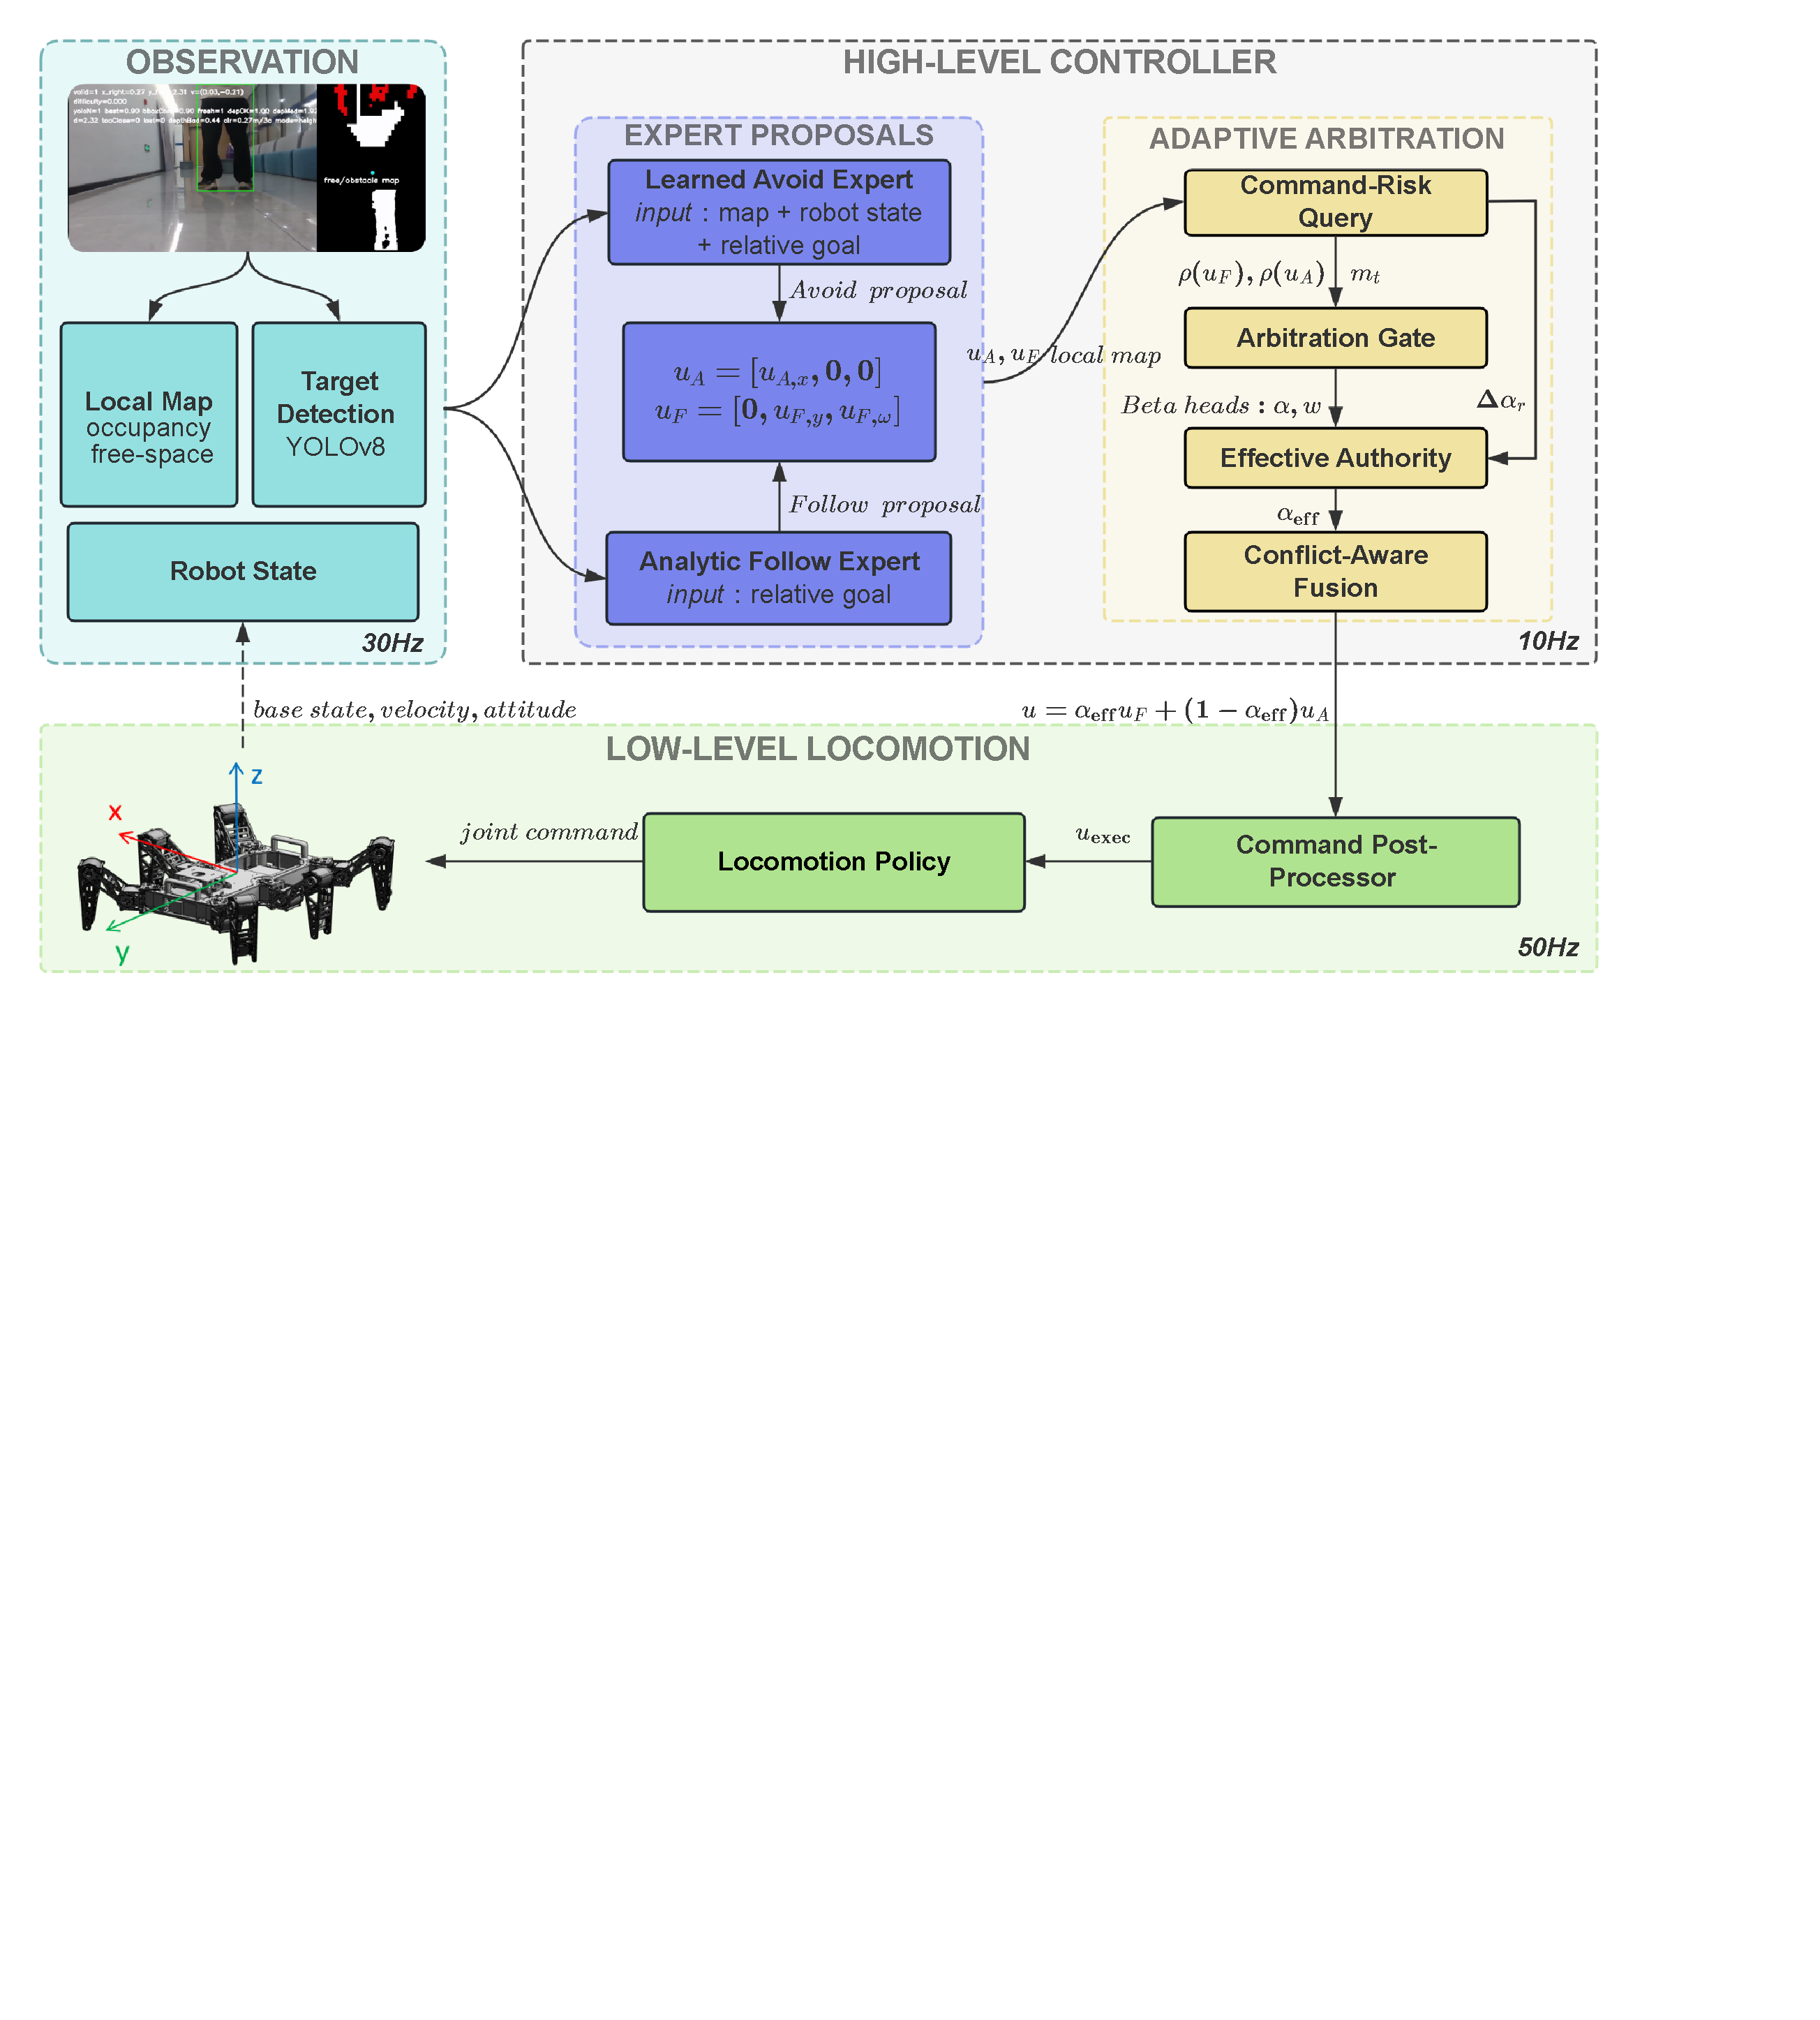
\includegraphics[trim=22.6bp 716.4bp 147.9bp 22.6bp,clip,width=0.90\textwidth]{figs/fig2_system.pdf}
\caption{Adaptive arbitration in command space. Onboard perception supplies a
local \rev{occupancy--free-space} map and relative target state
(YOLOv8). The analytic Follow expert proposes forward--yaw
motion, the learned Avoid expert proposes lateral motion, and directional
risk \rev{and its scalar memory} feed the arbitration gate. The gate computes
$\rev{\alphaeff}$ for command fusion before shared command post-processing and a
fixed locomotion policy. Rates indicate deployment frequencies: perception
30 Hz, arbitration 10 Hz, and locomotion 50 Hz.}
\label{fig:system}
\end{figure*}

\section{Method}
\label{sec:method}
The controller combines fixed locomotion, orthogonal expert proposals, and a learned arbitration gate (Fig.~\ref{fig:system}).

\textbf{A. Follow expert (analytic).}
The Follow expert computes $\uF=[0,u_{F,y},u_{F,\omega}]$ analytically
\rev{from the 2-D relative goal representing the target position relative to the robot}, using a turn-then-advance rule with
hysteresis: when the \rev{bearing magnitude} exceeds $0.35\,\mathrm{rad}$ the forward term
is suppressed and the robot turns in place; it resumes advancing once the
\rev{bearing magnitude} falls below $0.18\,\mathrm{rad}$.

\textbf{B. Avoid expert (learned).}
{\color{blue}
Avoid is pretrained independently in randomized obstacle layouts. Passage difficulty varies by stage, the environment supplies forward motion, and Follow is absent. The pretrained actor retains three command outputs, while arbitration uses only its lateral mean as the frozen Avoid proposal $\uA$ (observations and architecture: Sec.~IV-F, Table~\ref{tab:architecture}).

The reward encourages forward progress and improved directional clearance, penalizes the magnitude and variation of the lateral command, and adds a weak directional preference when both lateral alternatives are sufficiently clear. At $\Delta t=0.1\,\mathrm{s}$, the dense reward is
\begin{equation}
\begin{aligned}
r_t^A={}&\Delta y+0.03q_0(q_0-q_u)-0.005|u_x^{\mathrm{raw}}|\\
&-0.01|u_{x,t}^{\mathrm{exec}}-u_{x,t-1}^{\mathrm{exec}}|
+0.0005Gp\tfrac{u_x^{\mathrm{exec}}}{u_{x,\max}},
\end{aligned}
\label{eq:avoid_reward}
\end{equation}
where $\Delta y$ is forward displacement and $q_j=\mathrm{clip}((0.57-d_j)/0.57,0,1)$ for $j=0,u$. Distances $d_0,d_u$ use cones with a $25^\circ$ half-angle around the straight-ahead direction and the raw command direction on the same map before action execution. Superscripts raw/exec denote commands before/after processing; $u_{x,\max}$ is the lateral limit. The preference $p$ is the normalized lateral component of a valid forward goal direction. The indicator $G=1$ only beyond Avoid stage~1, with a valid preference, $\Delta y>0$, $d_0<0.57$, $d_L,d_R\ge0.57$, and $|d_L-d_R|\le0.10$ (distances in metres); otherwise $G=0$. Here $d_L,d_R$ query lateral commands $\pm u_{x,\max}$ combined with the supplied forward command. The reward does not use row indices, gap centers, or passage templates.

Terminal rewards replace $r_t^A$: $+2$ for the robot center crossing the layout's exit line without failure; $-20$ for collision, envelope intrusion, falling, or tilt/height violations, with failure taking precedence. Timeout ends the episode without the failure penalty. Lateral avoidance assumes that a feasible bypass is observable ahead.
\par}

\textbf{C. Directional command risk.}
\rev{The gate receives a two-channel robot-fixed local occupancy--free-space map, represented as a $32\times32$ grid covering a forward $3\,\mathrm{m}\times3\,\mathrm{m}$ region, with its origin at the camera mount. The occupancy channel marks occupied cells. The free-space channel is a dimensionless score formed by dilating occupancy with a $7\times7$ square kernel in simulation, deriving a free-space mask, taking its cellwise maximum with a $3\times3$ local average, then masking occupied and unobserved cells; it is not a metric distance field. The dilation radius was selected from physical measurements of the hexapod to account for its body dimensions and the additional lateral extent introduced by leg motion during locomotion. For each proposal with nonzero translation, distance $d$ from the map origin to the nearest occupied cell in the occupancy channel is queried within a cone centered at $\mathrm{atan2}(u_x,u_y)$ with a $25^\circ$ half-angle ($d=3.0\,\mathrm{m}$ when no occupied cell is observed in the cone). When translation is near zero, the simulation query falls back to the distance to the nearest occupied cell in the local map. Neither query evaluates swept yaw motion. Sidestepping can begin using bypass space observed ahead, but an empty query cone does not establish that the entire lateral path is clear.} Risk is
\begin{equation}
\rho(u)=1-\mathrm{clip}\!\left(\tfrac{d-d_{\mathrm{safe}}}
{d_{\mathrm{free}}-d_{\mathrm{safe}}},0,1\right),
\end{equation}
with $d_{\mathrm{safe}}=0.27\,\mathrm{m}$ and
$d_{\mathrm{free}}=0.57\,\mathrm{m}$. \rev{The fixed thresholds define a directional proximity score rather than clearance of the swept robot body. The $25^\circ$ half-angle is a fixed heuristic that defines the directional query neighborhood; no speed scaling or braking-distance model is used.}

For each proposal, $\rho_F=\rho(\uF)$ and $\rho_A=\rho(\uA)$. \emph{Risk memory with distance decay.} To retain recent hazards, scalar risk memory decays with forward body displacement, with no decay during pure lateral motion or stops:
\begin{equation}
\begin{aligned}
m_t &= \max\!\big(\rho_{F,t},m_{t-1}e^{-\Delta s/L_{\mathrm{clear}}}\big),\\
\Delta s &= \max(v_{y,t}^{\mathrm{body}},0)\,\Delta t,
\end{aligned}
\end{equation}
with $L_{\mathrm{clear}}=0.40\,\mathrm{m}$. This scalar is supplied to the
gate as a derived conflict feature. \rev{Instantaneous risk reflects current map observations; $m_t$ retains a scalar hazard signal, not an obstacle map.}

\textbf{D. Gate and conflict-aware fusion.}
A single arbitration gate uses Beta heads for the \rev{base Follow authority $\alpha\in(0,1)$}
and learned conflict variable $w\in(0,1)$. The gate combines local geometry, robot and target states, and conflict features derived from the proposals; the exact observations are specified in Sec.~IV-F.
The learned signed modulation and analytic risk correction
are
\begin{align}
\rev{\Delta\alpha_w} &= \lambda\,\mathrm{deadband}(2w-1),\quad
\rev{\Delta\alpha_r} = \gamma(\rAdir-\rFdir), \\
\rev{\alphaeff} &= \mathrm{clip}\!\left(\rev{\alpha}+\rev{\Delta\alpha_w}+\rev{\Delta\alpha_r},0,1\right),
\end{align}
with $\lambda=0.30$, $\gamma=0.15$, and
$\mathrm{deadband}(z)=z$ for $|z|>0.05$ and $0$ otherwise. The fused
command is
\begin{equation}
u = \rev{\alphaeff}\,\uF + (1-\rev{\alphaeff})\,\uA.
\label{eq:fusion}
\end{equation}
\rev{Outside the deadband,} values $w>0.5$ reinforce following, whereas $w<0.5$ suppresses it through
$\rev{\Delta\alpha_w}$. In the active unsaturated region,
$\partial\rev{\alphaeff}/\partial w=2\lambda=0.60$; it is zero inside the
dead zone or after clipping. \rev{The gains bound the learned and analytic corrections by $0.30$ and $0.15$, respectively, before clipping.}

\textbf{E. Low-level locomotion interface.}
The fixed locomotion policy tracks high-level commands at $50\,\mathrm{Hz}$ and is shared across methods. Before execution, all methods use the same amplitude clamping, slew-rate limiting \rev{to bound command changes}, and clearance-based scaling \rev{to attenuate translation near obstacles}.

\textbf{F. Training procedure.}
We first pretrain and freeze a hexapod locomotion policy conditioned on velocity commands with RSL-RL~\cite{ref:rudin}, using reward terms for camera stability and smooth impacts. With Avoid also frozen (Sec.~\ref{sec:method}-B), only the arbitration gate is trained. An auxiliary binary cross-entropy loss with weight $0.05$ encourages $w=0$ in states that clearly favor avoidance:
cases before row release satisfying $\rFdir>0.25$,
$\rFdir-\rAdir>0.05$, and command cosine $<0.5$, \rev{or global cases satisfying $\rFdir>0.45$, $\rFdir-\rAdir>0.15$, and command cosine $<0.3$.}

\rev{The Avoid expert, locomotion policy, and gate use the same hexapod asset in Isaac Gym~\cite{ref:isaac}; locomotion uses RSL-RL and the two learned high-level policies use PPO~\cite{ref:ppo}.} The curriculum has four levels and varies the number of obstacle rows from two to five together with target speed from $0.25$ to $0.50\msec$, with speed fixed within each episode. Over $120{,}000$ episodes, sampling shifts toward harder levels while retaining easier episodes. The five-row training layouts use two mirrored templates with alternating left/right passages and independent perturbations of obstacle positions up to $\pm0.06\,\mathrm{m}$; Sec.~V-A describes the held-out evaluation. Training obstacles are \rev{static, with a radius of $0.15\,\mathrm{m}$ and a height of $0.50\,\mathrm{m}$}; contact friction is randomized in $[0.4,0.8]$. During training, the policy receives a local \rev{occupancy--free-space} map rasterized from simulated obstacle geometry and restricted to the D435i stereo FOV rather than rendered depth.

\begin{table}[t]
\centering
\caption{\rev{Network architectures of the Avoid expert and arbitration gate. Both use the same map encoder architecture with independent weights; parameter counts include the critics used during training}}
\label{tab:architecture}
\setlength{\tabcolsep}{3pt}
\renewcommand{\arraystretch}{1.18}
\footnotesize
\color{blue}
\begin{tabular}{@{}>{\raggedright\arraybackslash}p{0.14\columnwidth}@{\hspace{4pt}}>{\raggedright\arraybackslash}p{0.41\columnwidth}@{\hspace{4pt}}>{\raggedright\arraybackslash}p{0.41\columnwidth}@{}}
\toprule
\textbf{Block} & \textbf{Avoid expert} & \textbf{Arbitration gate} \\
\midrule
Map encoder & \multicolumn{2}{>{\raggedright\arraybackslash}p{0.82\columnwidth}@{}}{2-ch local occupancy/free-space map + 2 normalized coordinate channels; Conv $4\to32\to64\to128$ ($3\times3$, strides $2/2/1$, pad 1, ELU); adaptive $4\times4$ average pooling; FC $2048\to128$.} \\
\addlinespace[2pt]
Scalar encoders & State MLP $14\!\to\!64\!\to\!64\!\to\!64$; goal MLP $2\!\to\!32\!\to\!32$ (ELU). & State MLP $13\!\to\!64\!\to\!64\!\to\!64$; goal/conflict MLP $18\!\to\!32\!\to\!32$ (ELU; 31 scalar inputs total). \\
\addlinespace[2pt]
Fusion & \multicolumn{2}{>{\raggedright\arraybackslash}p{0.82\columnwidth}@{}}{Concat. $128+64+32+1=225$; MLP $225\to256\to256$ (ELU). The 1-D difficulty input is fixed to zero for the evaluated gate.} \\
\addlinespace[2pt]
Actor head & Mean $256\to64\to3$; std $256\to64\to3$ (Softplus); lateral mean executed. & $4\times(256\to64\to1)$ Softplus concentration heads; two Beta distributions for $\alpha,w$; Beta means used at evaluation. \\
\addlinespace[2pt]
Critic / params & Value $256\to64\to1$; 1,029,575 params. & Value $256\to64\to1$; 1,063,237 params. \\
\bottomrule
\end{tabular}
\color{black}

\end{table}

\rev{Table~\ref{tab:architecture} summarizes the architectures; critics have separate encoders and trunks. The gate's 13-D robot state comprises planar position in world coordinates, yaw, body-frame planar velocity, yaw rate, height, roll/pitch, previous base authority $\alpha$, and the last command. Avoid fixes the authority entry to zero and appends imposed forward speed (14-D state); its map and 2-D relative goal are separate inputs. The gate's 18-D goal/conflict vector comprises the relative goal, Follow/Avoid proposals and their difference (9), risks $\rho_F,\rho_A$, risk memory $m_t$, translational command cosine $c$, conflict score $\max(\rho_F-\rho_A,0)(1-c)/2$, and two clearances normalized as $\mathrm{clip}(d/(3\,\mathrm{m}),0,1)$. Here $c=1$ if either translational proposal has norm at most $10^{-6}$.}


\rev{Both high-level stages use 1,000 iterations (12.288M interactions) each, for 24.576M in total; shared frozen locomotion training is excluded.} Gate PPO uses 256 environments with 48 steps per iteration; \rev{Avoid uses 512 environments with 24 steps.} The gate is optimized for five epochs per iteration with minibatches of 12,288, learning rate $6{\times}10^{-5}$, entropy coefficient 0.04, and clip ratio 0.05. Gate training combines row-progress, follow-distance,
success, and collision/failure\rev{/time} rewards with the $w$ auxiliary loss.
\rev{Information on row release supplies auxiliary training labels only; the actor
instead receives scalar risk memory.}

\textbf{G. Structural properties and scope.}
The raw blend lies in the proposals' convex hull. With $u_{\mathrm{nom}}=\rev{\alpha}\uF+(1-\rev{\alpha})\uA$ and $\delta u=u-u_{\mathrm{nom}}$,
\begin{equation}
\begin{aligned}
\delta u &= (\rev{\alphaeff}-\rev{\alpha})(\uF-\uA),\\
\|\delta u\| &\le (\lambda+\gamma)\|\uF-\uA\|.
\end{aligned}
\label{eq:residual_bound}
\end{equation}
Thus, the correction vanishes at coincident proposals and is bounded during conflict. \rev{These properties concern raw commands; they do not guarantee collision avoidance, since the set of safe executed motions need not be convex.}

\section{Experiments}
\textbf{A. Setup.}
\rev{Formal comparisons use a held-out five-row Stage-4 layout family excluded from Avoid/gate training, checkpoint selection, and parameter tuning. It preserves passability mismatch while breaking training's left/right alternation with successive passages on one side. The nominal row spacings extend beyond the range used in training. Each episode randomly perturbs obstacle positions around the nominal pattern. The nominal pattern has 15 obstacles (three per row) and a $0.75\,\mathrm{m}$ minimum passage width versus the robot's $\sim0.65\,\mathrm{m}$ leg-inclusive envelope. Tests use $0.35$, $0.50$, and $0.60\msec$; $0.60\msec$ is 20\% above the $0.50\msec$ training maximum.}
Main results are reported as mean $\pm$ SD over three evaluation seeds, with 128 episodes per seed (384 per method and speed; 50-s horizon). The hexapod has 18 actuated joints and a $0.25\,\mathrm{m}$ passing half-length. The D435i uses $87^\circ\times58^\circ$ depth FOV over $0.28$--$3.0\,\mathrm{m}$. Simulation uses structured geometric primitives; inference ablation and DWA use the same evaluation protocol. \rev{For Mono, curriculum probes use frozen checkpoints at levels 2--4 to diagnose training capability; these probes are separate from the formal held-out evaluation.} \rev{A separate sensitivity test across mixed difficulty levels shifted both nominal risk thresholds by $\pm0.05\,\mathrm{m}$ or varied $d_{\mathrm{free}}$ alone by $\pm0.10\,\mathrm{m}$, with the policy and post-processing fixed. Across three speeds (128 episodes per setting and speed), the pooled success and collision rates varied by 1.6 and 1.3 percentage points, respectively.}

\textbf{B. Compared methods.}
We organize the comparison into three groups.
\emph{(1) Arbitration ablations} share the experts, base sensor inputs, and
execution stack but apply different arbitration rules:
\emph{\rev{$\alpha$-only}} ($\rev{\alphaeff}=\rev{\alpha}$, no risk or learned modulation);
\emph{Geom-w}, a geometric clearance heuristic
$w_{\mathrm{geom}}=e^{-d/\tau}$ using the clearance $d$ along the Follow command and
$\tau=0.15\,\mathrm{m}$, with $\rev{\alphaeff}=\rev{\alpha}(1-w_{\mathrm{geom}})$;
\emph{Risk-only}, \rev{the learned base $\alpha$ plus analytic $\darisk$ term, with $\alpha_{\mathrm{eff}}=\mathrm{clip}(\alpha+\Delta\alpha_r,0,1)$, retrained from
scratch without $w$}; \emph{Rule-Override}, a reactive
override on $\rFdir-\rAdir$ that forces lateral avoidance by cutting the forward
command to as low as $10\%$ while retaining up to $70\%$ of the yaw
command, using one fixed parameter set across all speeds; and
\emph{\rev{Adaptive}}, the full proposed method.
\emph{(2) Structural alternatives.} \emph{Additive-Fusion} replaces the
gate with direct command addition, $u=\uF+\uA$, keeping the same experts
but with no gate. \rev{Fixed-Authority uses
$u=\alpha^*\uF+(1-\alpha^*)\uA$ with a global constant
$\alpha^*=0.50$ selected from a 21-point validation sweep over $[0,1]$ by maximizing mean task success across separate validation trials at $0.35$ and $0.50\msec$, then held fixed across speeds, with the same experts, post-processing, and locomotion policy.}
\emph{(3) External alternatives} (Sec.~\ref{sec:external}): a \emph{monolithic PPO} policy and a \emph{DWA-style velocity search}, both using the \rev{same base map, robot state, and target sensor inputs}, command limits, and fixed low-level stack.

\textbf{C. Metrics.}
Task success is the event-level criterion of Sec.~III-D; we report collision
rate and progress toward final-row clearance as trajectory diagnostics,
plus follow-distance MAE and L2 where target retention is relevant. \rev{Row progress is the fraction of obstacle rows safely completed, distinct from the binary final-row-clearance indicator L3.}

\section{Results}
\label{sec:results}
All simulation results use the event-level success definition of
Sec.~III-D; their evaluation protocols are specified in Sec.~V-A.

\textbf{A. Main performance.}
At high conflict, Adaptive combines high task success with low collision (Table~\ref{tab:main}; Fig.~\ref{fig:main}). \rev{Fig.~\ref{fig:simtraj}(a) shows a scene from the training distribution, distinct from the formal evaluation layout.} At $0.60\msec$, success is $95.3\%$, collision is $3.9\%$, and follow-distance MAE is $0.62\,\mathrm{m}$.

\rev{The arbitration variants degrade differently as target speed increases. Although $\alpha$-only learns a context-dependent base authority, its task success falls to zero at the two higher speeds. Geom-w and Risk-only remain effective at the intermediate speed, but at $0.60\msec$ their lower collision rates than $\alpha$-only coexist with near-zero task success and large follow-distance errors. Rule-Override retains substantial task success but incurs frequent collisions. Across these variants, task failure appears through different combinations of collision and follow-distance error.}



\begin{figure}[t]
\centering
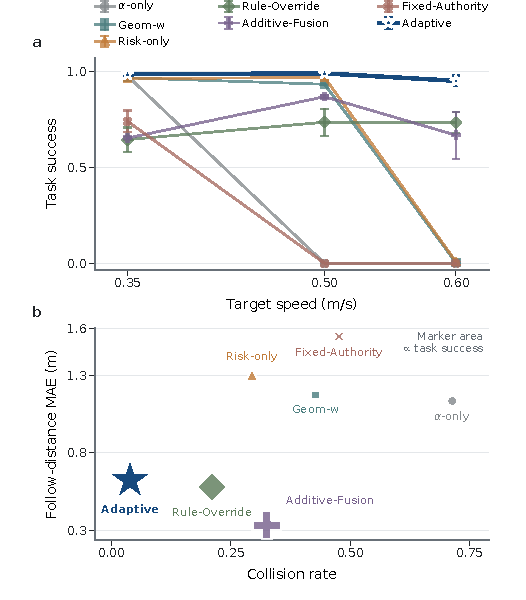
\includegraphics[width=\columnwidth,trim=12bp 5bp 14bp 0bp,clip]{figs/final_main_performance_nature.pdf}
\caption{Main performance on the \rev{held-out Stage-4 evaluation}. (a) Task success versus target speed. (b) Follow-distance MAE versus collision rate at $0.60\msec$; marker area encodes task success.}
\label{fig:main}
\end{figure}

\begin{figure*}[t]
\centering
\begin{minipage}[c]{0.41\textwidth}
\centering
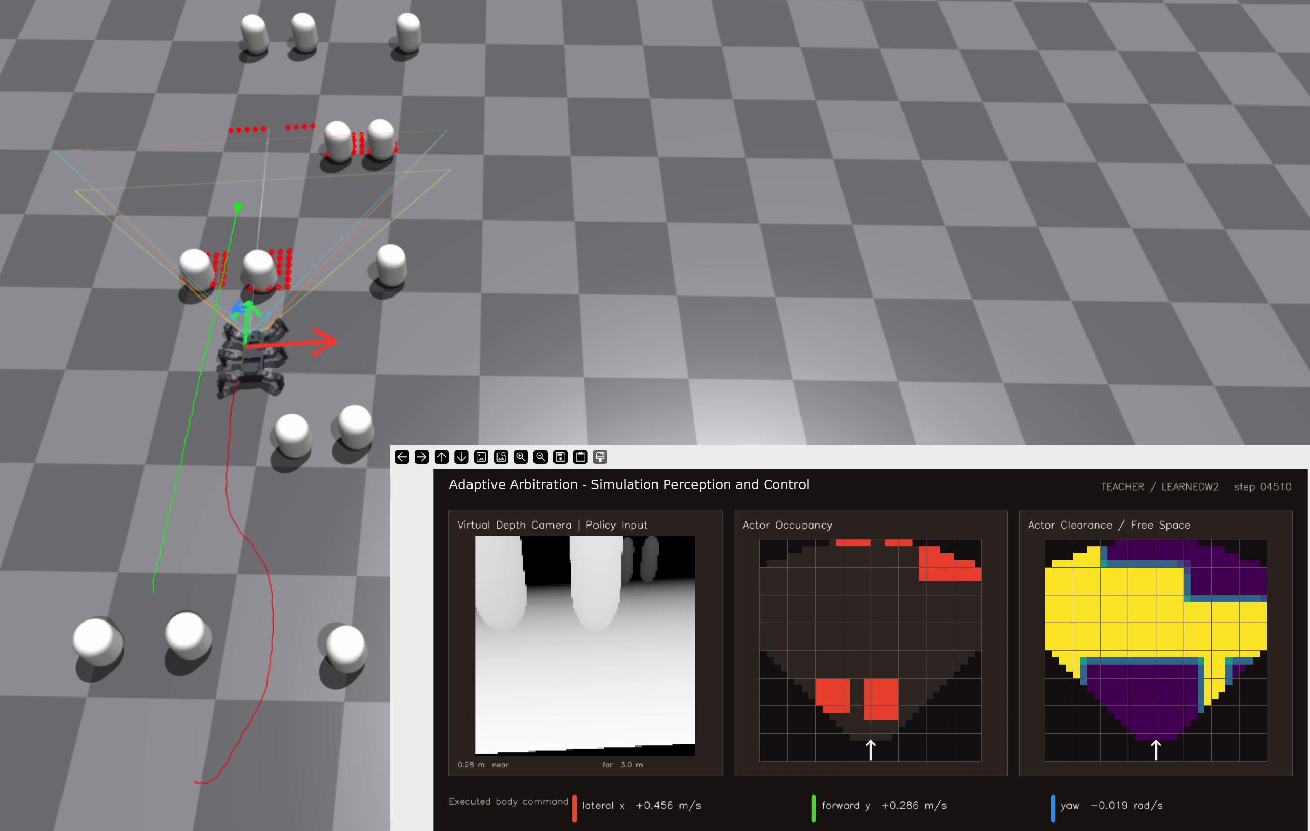
\includegraphics[width=\linewidth]{figs/fig5_sim_overview_crop_adaptive.pdf}\\[-0.8mm]
{\scriptsize (a)}
\end{minipage}\hfill
\begin{minipage}[c]{0.55\textwidth}
\centering
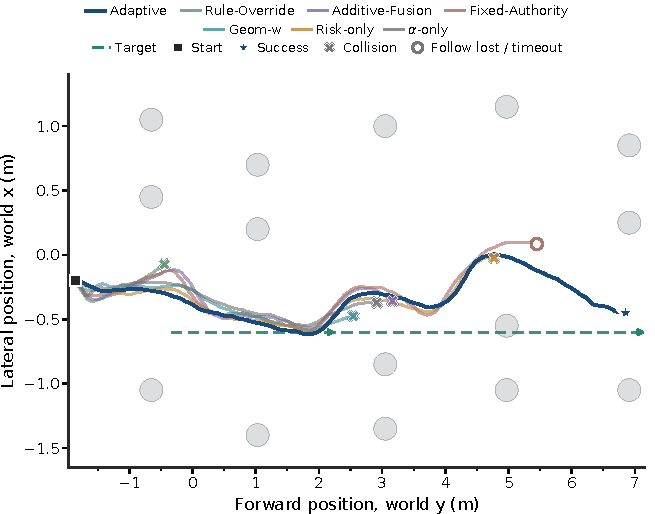
\includegraphics[width=\linewidth]{figs/revision_heldout_mixed_v1_all_methods_trajectories_nature_refined.pdf}\\[-0.8mm]
{\scriptsize (b)}
\end{minipage}
\caption{\rev{Training and evaluation scenes. (a) Representative training scene and policy inputs. (b) Representative trajectories at $0.60\msec$; obstacles show the nominal geometry of the held-out Stage-4 layout.}}
\label{fig:simtraj}
\end{figure*}

\begin{figure}[!b]
\centering
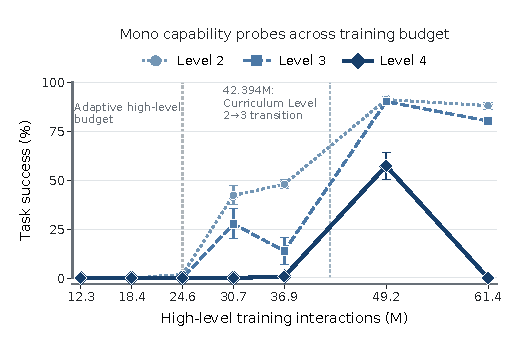
\includegraphics[width=\columnwidth]{figs/fig_mono_budget_capability_vertical.pdf}
\caption{\rev{Mono capability emergence. Probes use frozen checkpoints at curriculum levels 2--4 and $0.35\msec$, with policy updates disabled. Error bars show sample SD across three evaluation seeds for one training seed; the vertical lines mark the Adaptive budget and curriculum transition.}}
\label{fig:mono}
\end{figure}

\begin{figure}[!b]
\centering
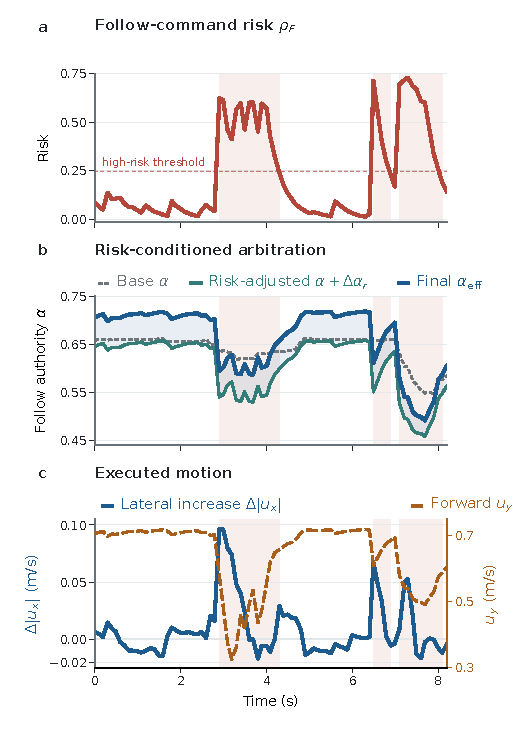
\includegraphics[width=\columnwidth]{figs/final_real_robot_arbitration_nature.pdf}
\caption{Representative real-robot arbitration. (a) Risk derived from stereo depth peaks during conflict. \rev{(b) The analytic risk term reduces Follow authority; blue shading shows its partial restoration by the learned correction.} (c) Forward and lateral motion; \rev{$\Delta|u_x|$ is relative to the pre-conflict median.}}
\label{fig:real_arbitration}
\end{figure}

\begin{figure*}[!tb]
\centering
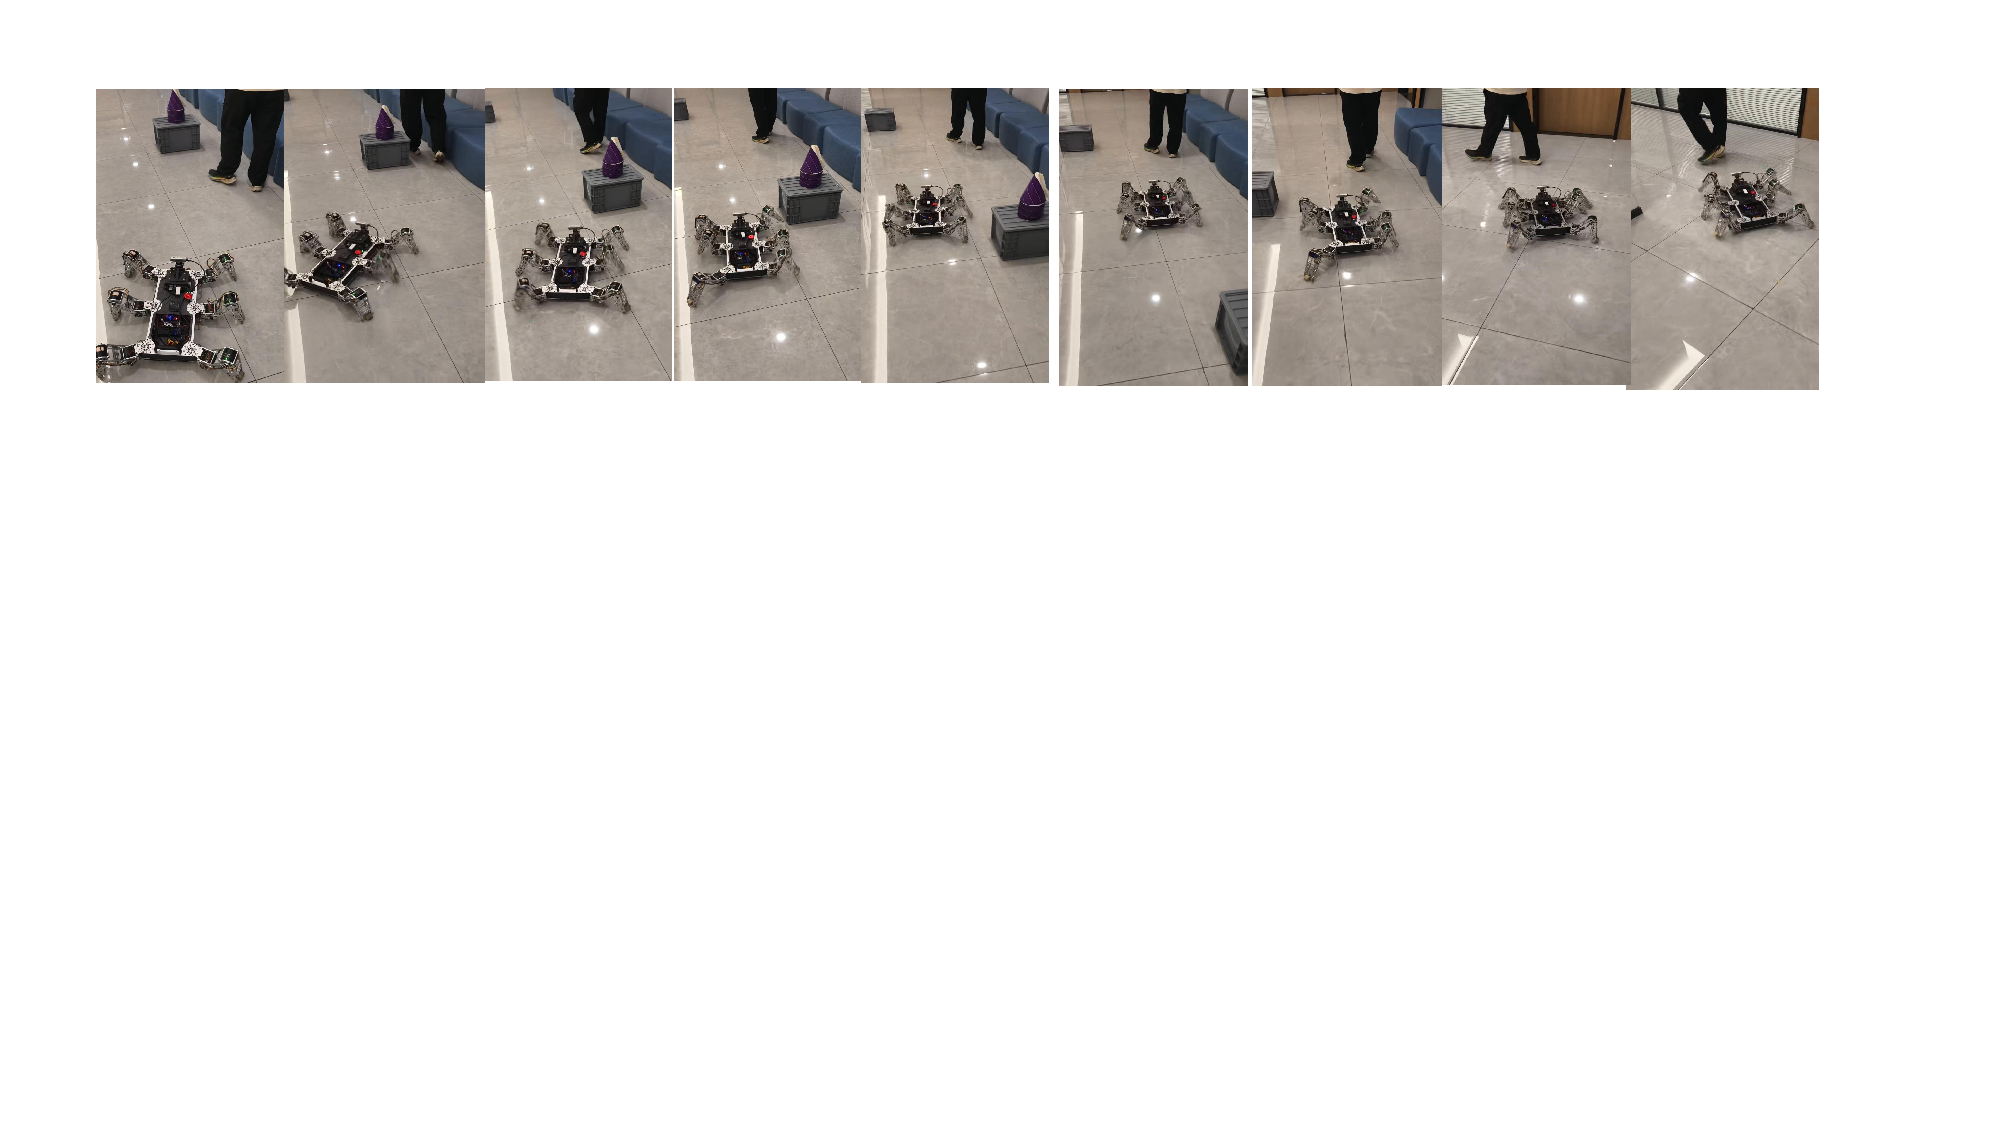
\includegraphics[width=\textwidth]{figs/fig4a_real_follow.pdf}\\[-1.8mm]
{\scriptsize (a)}\\[-0.2mm]

\includegraphics[width=\textwidth]{figs/revision_real_onboard.pdf}\\[-1.8mm]
{\scriptsize (b)}
\caption{Real-robot deployment views. (a) The hexapod follows the walking
target while sidestepping around staggered corridor obstacles. \rev{(b) Three representative onboard times (frames 1, 3, and 5)} show the target
state and local \rev{occupancy--free-space} map derived from stereo depth and used by Adaptive.}
\label{fig:real_views}
\end{figure*}

\begin{table}[t]
\centering
\caption{\rev{Performance on the held-out Stage-4 evaluation.} Values are mean $\pm$ SD; speed in m/s. \rev{Bold marks the best mean per speed and metric}}
\label{tab:main}
\setlength{\tabcolsep}{1.75pt}
\renewcommand{\arraystretch}{1.18}
\renewcommand{\ms}[2]{\ensuremath{#1{\pm}#2}}
\scriptsize
\begin{tabular}{@{}llcccc@{}}
\toprule
Spd. & Method & Succ. [\%] $\uparrow$ & Row prog. [\%] $\uparrow$ & Coll. [\%] $\downarrow$ & MAE [m] $\downarrow$ \\
\midrule
\multirow{7}{*}{\rotatebox{90}{$0.35$}} & \rev{$\alpha$-only} & \ms{97.9}{0.5} & \ms{99.6}{0.1} & \ms{2.1}{0.5} & \ms{0.217}{0.001} \\
 & Geom-w & \ms{96.9}{1.4} & \ms{99.2}{0.6} & \ms{3.1}{1.4} & \ms{0.171}{0.001} \\
 & Risk-only & \ms{96.4}{1.2} & \ms{99.3}{0.2} & \ms{3.6}{1.2} & \ms{0.164}{0.001} \\
 & Rule-Override & \ms{64.6}{6.3} & \ms{82.1}{4.0} & \ms{34.6}{6.6} & \ms{0.164}{0.008} \\
 & Additive-Fusion & \ms{65.4}{1.2} & \ms{84.2}{1.0} & \ms{34.4}{1.4} & \ms{\mathbf{0.102}}{0.001} \\
 & \rev{Fixed-Authority} & \rev{\ms{74.2}{5.6}} & \rev{\ms{89.9}{3.0}} & \rev{\ms{24.5}{6.1}} & \rev{\ms{0.390}{0.009}} \\
 & \textbf{\rev{Adaptive}} & \ms{\mathbf{98.7}}{0.9} & \ms{\mathbf{99.8}}{0.1} & \ms{\mathbf{1.3}}{0.9} & \ms{0.120}{0.000} \\
\midrule
\multirow{7}{*}{\rotatebox{90}{$0.50$}} & \rev{$\alpha$-only} & \ms{0.0}{0.0} & \ms{93.0}{1.2} & \ms{30.7}{6.4} & \ms{0.969}{0.035} \\
 & Geom-w & \ms{93.5}{0.5} & \ms{97.2}{0.7} & \ms{6.5}{0.5} & \ms{0.430}{0.001} \\
 & Risk-only & \ms{97.1}{0.9} & \ms{99.0}{0.5} & \ms{2.9}{0.9} & \ms{0.405}{0.001} \\
 & Rule-Override & \ms{73.7}{7.1} & \ms{90.0}{2.8} & \ms{24.7}{7.3} & \ms{0.381}{0.013} \\
 & Additive-Fusion & \ms{87.0}{0.9} & \ms{94.6}{0.4} & \ms{12.5}{0.8} & \ms{\mathbf{0.177}}{0.002} \\
 & \rev{Fixed-Authority} & \rev{\ms{0.0}{0.0}} & \rev{\ms{43.6}{0.5}} & \rev{\ms{50.8}{4.1}} & \rev{\ms{1.220}{0.020}} \\
 & \textbf{\rev{Adaptive}} & \ms{\mathbf{99.2}}{0.8} & \ms{\mathbf{99.9}}{0.2} & \ms{\mathbf{0.8}}{0.8} & \ms{0.355}{0.003} \\
\midrule
\multirow{7}{*}{\rotatebox{90}{$0.60$}} & \rev{$\alpha$-only} & \ms{0.0}{0.0} & \ms{79.4}{0.9} & \ms{71.4}{3.6} & \ms{1.133}{0.012} \\
 & Geom-w & \ms{0.3}{0.5} & \ms{74.6}{1.8} & \ms{42.7}{8.4} & \ms{1.172}{0.015} \\
 & Risk-only & \ms{0.8}{0.8} & \ms{71.5}{0.2} & \ms{29.4}{7.1} & \ms{1.305}{0.031} \\
 & Rule-Override & \ms{73.4}{5.5} & \ms{86.1}{2.7} & \ms{21.1}{4.8} & \ms{0.582}{0.019} \\
 & Additive-Fusion & \ms{66.9}{12.3} & \ms{87.4}{5.0} & \ms{32.6}{12.6} & \ms{\mathbf{0.334}}{0.040} \\
 & \rev{Fixed-Authority} & \rev{\ms{0.0}{0.0}} & \rev{\ms{39.9}{0.1}} & \rev{\ms{47.7}{2.8}} & \rev{\ms{1.549}{0.004}} \\
 & \textbf{\rev{Adaptive}} & \ms{\mathbf{95.3}}{2.8} & \ms{\mathbf{98.5}}{0.8} & \ms{\mathbf{3.9}}{2.7} & \ms{0.623}{0.004} \\
\bottomrule
\end{tabular}
\end{table}





\textbf{B. Inference ablation.}
Table~\ref{tab:mech} reuses the Adaptive checkpoint while setting $\rev{\Delta\alpha_w}=0$ only at inference. \rev{Success remains high at $0.35$ and $0.50\msec$, but falls to zero at $0.60\msec$ despite substantial row progress, while follow-distance MAE rises to $1.46\,\mathrm{m}$.  With the experts and policy checkpoint fixed, this comparison supports the learned correction's role in sustaining target following under the highest tested conflict. Avoid and the gate observe body-frame velocity, while Follow responds to the relative target state; the highest speed therefore stresses the complete system.}

\begin{table}[t]
\centering
\caption{Ablation of the learned correction ($\rev{\Delta\alpha_w}=0$ at inference). \rev{Success, row progress, and collision are proportions; speed is in m/s}}
\label{tab:mech}
\setlength{\tabcolsep}{2.5pt}
\footnotesize
\begin{tabular}{lccccc}
\toprule
Spd. & Success $\uparrow$ & Row prog. $\uparrow$ & Coll. $\downarrow$ & MAE [m] $\downarrow$ &
$\rev{\Delta\alpha_w}$ (pred.) \\
\midrule
$0.35$ & $0.974$ & $0.993$ & $0.023$ & $0.176$ & $0.066$ \\
$0.50$ & $0.982$ & $0.992$ & $0.016$ & $0.438$ & $0.067$ \\
$0.60$ & $0.000$ & $0.739$ & $0.133$ & $1.463$ & $0.066$ \\
\bottomrule
\end{tabular}
\end{table}

\rev{\textbf{C. Structural alternatives.}}
\rev{Additive-Fusion maintains low follow-distance error but incurs substantially more collisions, exposing an unresolved safety--following trade-off. Fixed-Authority fails to complete the task at the higher speeds, indicating the limits of one global allocation across conditions.}
\rev{Representative trajectories are shown in Fig.~\ref{fig:simtraj}(b).}

\textbf{D. External alternatives.}
\phantomsection\label{sec:external}
We compare against Monolithic PPO as the primary learning baseline and a DWA-style velocity search as a planning baseline; both use the same command interface and target information as Adaptive.

\emph{Monolithic PPO.} The policy outputs the complete high-level command without Follow/Avoid decomposition. \rev{It shares the base observations, spatial map encoder family, command limits, post-processing, and frozen locomotion with Adaptive. Mono and the gate have similar actor--critic parameter counts (1.03M vs. 1.06M), while Adaptive additionally uses the frozen Avoid expert. Mono is trained for up to 61.4M interactions under a curriculum whose progression depends on task performance, with one training seed and three evaluation seeds.}

\rev{At the matched 24.6M budget, Mono has zero task success at all three speeds, whereas Adaptive exceeds $95\%$ (Table~\ref{tab:mono}). Extended training raises Mono to $94.5\%$ success at $0.50\msec$, confirming that the complete task is learnable without expert decomposition. Performance nevertheless remains uneven in this training run: at $0.35\msec$, within the training range, success falls from $57.3\%$ at 49.2M interactions to zero at 61.4M. At 49.2M and $0.60\msec$, $60.4\%$ of episodes complete all rows without collision, yet task success remains zero and follow-distance MAE reaches $1.25\,\mathrm{m}$. Thus, obstacle traversal can be acquired without consistently satisfying the following objective.}

\begin{table}[t]
\centering
\caption{\rev{Held-out Stage-4 task success (\%); speeds in m/s}}
\label{tab:mono}
\setlength{\tabcolsep}{2.5pt}
\footnotesize
\begingroup\color{blue}
\begin{tabular}{lcccc}
\toprule
Policy & Budget (M) & 0.35 & 0.50 & 0.60 \\
\midrule
Adaptive & 24.576 & \ms{98.7}{0.9} & \ms{99.2}{0.8} & \ms{95.3}{2.8} \\
Mono 2000 & 24.576 & \ms{0.0}{0.0} & \ms{0.0}{0.0} & \ms{0.0}{0.0} \\
Mono 4000 & 49.152 & \ms{57.3}{6.7} & \ms{94.5}{0.0} & \ms{0.0}{0.0} \\
Mono 5000 & 61.440 & \ms{0.0}{0.0} & \ms{93.0}{2.7} & \ms{1.3}{0.9} \\
\bottomrule
\end{tabular}
\endgroup
\par\vspace{1pt}\noindent{\scriptsize\color{blue}Adaptive: 12.288M Avoid + 12.288M gate interactions (shared low-level training excluded); Mono uses one training seed. Entries are mean $\pm$ sample SD over three evaluation seeds; each Mono row uses the same checkpoint across speeds.}
\end{table}







\emph{DWA-style velocity search.} DWA uses the same map, target, command limits, post-processor, and low-level policy as Adaptive. It searches reachable commands at 10 Hz, scoring collision, risk, target distance and bearing, progress, and smoothness. Tuning on validation trials selected a $7\times5\times5$ grid and $1.2\,\mathrm{s}$ horizon. The best tested setting achieves $8.2\%$ success at $0.35\msec$ and zero at $0.60\msec$ (Table~\ref{tab:dwa}). \rev{Across the tested cost settings, changes in obstacle progress and following error do not yield both low collision and high task success.}

\begin{table}[t]
\centering
\caption{DWA-style velocity search}
\label{tab:dwa}
\setlength{\tabcolsep}{3pt}
\footnotesize
\begin{tabular}{llcccc}
\toprule
Search bias & Spd. & Success $\uparrow$ & Coll. $\downarrow$ &
Row prog. $\uparrow$ & MAE [m] $\downarrow$ \\
\midrule
\multirow{2}{*}{Safety-biased}
 & $0.35$ & $0.053$ & $0.612$ & $0.138$ & $0.678$ \\
 & $0.60$ & $0.000$ & $0.838$ & $0.000$ & $1.028$ \\
\multirow{2}{*}{Balanced}
 & $0.35$ & $0.026$ & $0.938$ & $0.188$ & $0.375$ \\
 & $0.60$ & $0.000$ & $0.969$ & $0.375$ & $0.592$ \\
\multirow{2}{*}{Tracking-biased}
 & $0.35$ & $0.082$ & $0.744$ & $0.344$ & $0.528$ \\
 & $0.60$ & $0.000$ & $0.881$ & $0.500$ & $0.690$ \\
\bottomrule
\end{tabular}
\end{table}

\textbf{E. Real-robot deployment.}
We deploy the policy on a hexapod in a narrow indoor corridor with two
staggered obstacle rows. Their passable gaps alternate left and right, so the
robot must sidestep through each row while keeping the walking person in view. Hardware rows replace the regular
simulated primitives with boxes and cones, testing transfer beyond
the simulated obstacle representation.
YOLOv8 \rev{is used only for target detection and relative goal estimation; obstacle geometry is derived from stereo depth after masking depth points associated with the detected target. The remaining valid depth points are back-projected using camera intrinsics, transformed to robot-aligned coordinates, filtered by height, and rasterized into the occupancy channel of the local map. The local map is updated from current and short-term depth observations in the robot-fixed frame, while $m_t$ separately retains scalar risk history. No persistent global obstacle map is maintained.} Simulation uses actor rasterization in place of stereo depth.
\rev{Adaptive and Rule-Override use identical target detection, local map generation, and perception settings.} \rev{Under the staggered-row protocol, Adaptive achieves higher task success (Table~\ref{tab:real}) and lower mean follow-distance MAE than Rule-Override ($0.52$ versus $1.21\,\mathrm{m}$).}
Fig.~\ref{fig:real_arbitration} shows a representative arbitration trace; Fig.~\ref{fig:real_views} shows the real-robot and onboard views.

A sharp-turn corridor joins two row segments at $90^\circ$. Adaptive succeeds in $18/20$ trials without scene-specific switching, bringing its overall success to $37/40$ across both scenes (Table~\ref{tab:real}). \rev{The three Adaptive failures comprise two obstacle contacts and one target loss. Either event makes the trial unsuccessful; subsequent recovery does not change this classification.} The supplementary video shows the sequence.

\begin{table}[t]
\centering
\caption{Real-robot results (60 trials)}
\label{tab:real}
\footnotesize
\setlength{\tabcolsep}{3pt}
\begin{tabular*}{\columnwidth}{@{\extracolsep{\fill}}llccccc@{}}
\toprule
Method & Scene & Trials & Success & Coll. & Lost & Rate \\
\midrule
\rev{Adaptive} & Staggered rows & $20$ & $19$ & $1$ & $0$ & $95\%$ \\
Rule-Override & Staggered rows & $20$ & $12$ & $6$ & $2$ & $60\%$ \\
\rev{Adaptive} & Sharp target turn & $20$ & $18$ & $1$ & $1$ & $90\%$ \\
\rev{Adaptive} & Overall & $40$ & $37$ & $2$ & $1$ & $92.5\%$ \\
\bottomrule
\end{tabular*}
\end{table}

\section{Discussion and Limitations}
\rev{\textbf{Role of adaptive arbitration.}} \rev{Lower collision rates, substantial obstacle progress, and low follow-distance error can each coexist with task failure. With the experts fixed, arbitration variants show different coordination failure patterns. More directly, disabling the learned correction in the same Adaptive checkpoint reduces task success to zero at the highest tested speed. Mono confirms that the complete task is learnable without expert decomposition, but its evaluated run does not consistently maintain obstacle traversal and sustained following together across speeds. These findings support learning how authority should change with context.}

\textbf{Scope and limitations.} \rev{Lateral-only Avoid assumes a feasible bypass observable in the forward map. The evaluated obstacles are static; interaction with dynamic obstacles is outside the present scope. Solid transverse walls, dead ends, concave traps, or a target stopping before a barrier may require stopping, backward motion, or higher-level replanning; the evaluated controller has no dedicated dead-end recovery or global replanning mechanism. Directional risk measures proximity rather than swept-footprint clearance, and the bounded convex blend does not certify collision-free execution.}

\section{Conclusion}
\rev{We presented adaptive command-space arbitration for target following under passability mismatch, focusing learning on the coordination of fixed Follow and Avoid proposals. Controlled comparisons show that Additive-Fusion and Fixed-Authority do not maintain comparable task performance across the tested conditions, while extended Monolithic PPO training confirms that the complete task can be learned without expert decomposition. Adaptive achieves $95.3\%$ success on the held-out evaluation at $0.60\,\mathrm{m/s}$ and succeeds in 37 of 40 hardware trials across staggered-row and sharp-turn corridors. Together, these results support context-dependent authority allocation for balancing obstacle negotiation with sustained target following in the tested conditions.}

\FloatBarrier
\begin{thebibliography}{99}
\setlength{\itemsep}{-1.2pt}
\bibitem{ref:personfollowing} M.~J. Islam, J.~Hong, and J.~Sattar,
``Person-following by autonomous robots: A categorical overview,'' \emph{The
International Journal of Robotics Research}, vol.~38, no.~14, pp.~1581--1618,
2019.
\bibitem{ref:socialfollow} \rev{J.~Montesdeoca, J.~M.~Toibero, J.~Jordan, A.~Zell, and R.~Carelli,
``Person-following controller with socially acceptable robot motion,''
\emph{Robotics and Autonomous Systems}, vol.~153, Art. no.~104075, 2022.}
\bibitem{ref:abs} T.~He, C.~Zhang, W.~Xiao, G.~He, C.~Liu, and G.~Shi,
``Agile but safe: Learning collision-free high-speed legged locomotion,'' in
\emph{Robotics: Science and Systems (RSS)}, 2024.
\bibitem{ref:miki} T.~Miki, J.~Lee, J.~Hwangbo, L.~Wellhausen, V.~Koltun,
and M.~Hutter, ``Learning robust perceptive locomotion for quadrupedal
robots in the wild,'' \emph{Science Robotics}, vol.~7, no.~62, p.~eabk2822,
2022.
\bibitem{ref:dwa} D.~Fox, W.~Burgard, and S.~Thrun, ``The dynamic window
approach to collision avoidance,'' \emph{IEEE Robotics \& Automation
Magazine}, vol.~4, no.~1, pp.~23--33, 1997.
\bibitem{ref:cbf} A.~D. Ames, X.~Xu, J.~W. Grizzle, and P.~Tabuada,
``Control barrier function based quadratic programs for safety critical
systems,'' \emph{IEEE Transactions on Automatic Control}, vol.~62, no.~8,
pp.~3861--3876, 2017.
\bibitem{ref:cpo} \rev{J.~Achiam, D.~Held, A.~Tamar, and P.~Abbeel,
``Constrained policy optimization,'' in \emph{Proceedings of the 34th
International Conference on Machine Learning}, PMLR, vol.~70, pp.~22--31,
2017.}
\bibitem{ref:moe} R.~A. Jacobs, M.~I. Jordan, S.~J. Nowlan, and
G.~E. Hinton, ``Adaptive mixtures of local experts,'' \emph{Neural
Computation}, vol.~3, no.~1, pp.~79--87, 1991.
\bibitem{ref:mela} \rev{C.~Yang, K.~Yuan, Q.~Zhu, W.~Yu, and Z.~Li,
``Multi-expert learning of adaptive legged locomotion,''
\emph{Science Robotics}, vol.~5, no.~49, Art. no.~eabb2174, 2020.}
\bibitem{ref:leaderfollow} C.~Scheidemann \emph{et al.},
``Obstacle-avoidant leader following with a quadruped robot,'' in
\emph{2025 IEEE International Conference on Robotics and Automation (ICRA)},
2025, pp.~1407--1413.
\bibitem{ref:policyblend} A.~D. Dragan and S.~S. Srinivasa, ``A
policy-blending formalism for shared control,'' \emph{The International
Journal of Robotics Research}, vol.~32, no.~7, pp.~790--805, 2013.
\bibitem{ref:residualrl} T.~Johannink \emph{et al.}, ``Residual reinforcement
learning for robot control,'' in \emph{2019 IEEE International Conference on
Robotics and Automation (ICRA)}, 2019, pp.~6023--6029.
\bibitem{ref:rudin} N.~Rudin, D.~Hoeller, P.~Reist, and M.~Hutter,
``Learning to walk in minutes using massively parallel deep reinforcement
learning,'' in \emph{Proceedings of the 5th Conference on Robot Learning
(CoRL)}, 2022, pp.~91--100.
\bibitem{ref:isaac} V.~Makoviychuk \emph{et al.}, ``Isaac Gym:
High-performance GPU-based physics simulation for robot learning,'' in
\emph{NeurIPS Datasets and Benchmarks Track}, 2021.
\bibitem{ref:ppo} J.~Schulman, F.~Wolski, P.~Dhariwal, A.~Radford, and
O.~Klimov, ``Proximal policy optimization algorithms,'' \emph{arXiv
preprint arXiv:1707.06347}, 2017.
\end{thebibliography}

\end{document}
